% Created 2026-10-22 Thu 01:04
% Intended LaTeX compiler: pdflatex
\documentclass[presentation, aspectratio=169]{beamer}

\usepackage[utf8x]{inputenc}
\usepackage[T1]{fontenc}
\usepackage{graphicx}
\usepackage{longtable}
\usepackage{wrapfig}
\usepackage{rotating}
\usepackage[normalem]{ulem}
\usepackage{amsmath}
\usepackage{amssymb}
\usepackage{capt-of}
\usepackage{hyperref}
\usepackage{palatino}
\usepackage{booktabs}
\setbeamerfont{title}{size=\large}
\setbeamerfont{author}{size=\small}
\usetheme[numbering=fraction, progressbar=frametitle]{metropolis}
\author{Lucas Mello Schnorr, Vinícius Garcia Pinto, Raymond Namyst, Samuel Thibault}
\date{SSCAD 2026 --- Minicurso 3 --- \url{https://github.com/schnorr/starpu-tutorial}}
\title{Development of Parallel Applications with the Task-Based Paradigm and the StarPU Runtime}
\begin{document}

\setbeamertemplate{navigation symbols}{}
\maketitle
\section{Opening}
\label{sec:orgaf229b2}

\begin{frame}[label={sec:orgcdcca3f},fragile]{Today, 14:00--16:10, no break}
 \begin{center}
\begin{tabular}{llll}
14:00 & 10 min & Opening, start the containers & \\
14:10 & 15 min & Concepts: tasks, DAG, STF & exposition\\
14:25 & 15 min & \alert{Hands-on 1}: first programs & \texttt{hello\_world}, \texttt{vector\_scal}\\
14:40 & 15 min & The StarPU runtime & exposition\\
14:55 & 30 min & \alert{Hands-on 2}: tiled GEMM & \texttt{gemm\_starpu}, GPU demo\\
15:25 & 10 min & Observing executions & exposition\\
15:35 & 25 min & \alert{Hands-on 3}: traces and StarVZ & \texttt{starvz}\\
16:00 & 10 min & Closing, questions & \\
\end{tabular}
\end{center}

Everything is in the companion repository and in the book chapter.
\end{frame}
\begin{frame}[label={sec:org2aa901c},fragile]{Start the StarPU container now}
 First load the two images (handout, "Opening": from the archives
distributed in the room, or with \texttt{podman pull}). Then:

\footnotesize
\begin{verbatim}
git clone https://github.com/schnorr/starpu-tutorial.git
cd starpu-tutorial
podman run -it --userns=keep-id \
    --mount type=bind,src="$(pwd)",target=/home/starpu/mount \
    registry.gitlab.inria.fr/starpu/starpu-docker/starpu:latest
# inside the container
starpu_machine_display -notopology
\end{verbatim}
\normalsize

You should see one CPU worker per core. Keep this shell open.
\end{frame}
\section{Concepts: tasks, DAG, STF}
\label{sec:org135560f}

\begin{frame}[label={sec:org22652fd}]{A typical HPC node}
\begin{itemize}
\item One or more multicore processors, one or more GPUs.
\item Each GPU has its own \alert{device memory}, linked to the \alert{host memory}
by PCIe: 16 GB/s (PCIe 3.0 x16) to 63 GB/s (PCIe 5.0 x16).
\item The bus is much slower than either memory.
\end{itemize}

Goal: compute \(C \leftarrow C + A B\) using \alert{every} core and the GPU.
\end{frame}
\begin{frame}[label={sec:org2ee299c},fragile]{Programming it by hand}
 \scriptsize
\begin{verbatim}
unsigned jgpu = NB * 0.8;  /* GPU share: tuned by hand for this node */
cudaMemcpy(dA, A, ...); cudaMemcpy(dB, B, ...); cudaMemcpy(dC, C, ...);
cublasSgemm(handle, ..., gpu_cols, ...);              /* asynchronous */
omp_set_num_threads(ncores - 1);    /* one core drives the GPU */
#pragma omp parallel for collapse(2) proc_bind(close)
for (unsigned j = jgpu; j < NB; j++)
    for (unsigned i = 0; i < NB; i++)
        for (unsigned k = 0; k < NB; k++)
            gemm_block(BS, N, BLK(A, i, k), BLK(B, k, j), BLK(C, i, j));
cudaMemcpy(C, dC, ...);
\end{verbatim}
\normalsize

Every line hides a decision valid for one machine only:
\begin{enumerate}
\item \alert{balancing} the work, 2. \alert{managing} memory transfers,
\item \alert{pinning} threads, 4. \alert{porting} to another node.
\end{enumerate}
\end{frame}
\begin{frame}[label={sec:org16ef3b7}]{The task-based paradigm}
\begin{itemize}
\item The programmer describes \alert{what}: tasks, the data they access, and
how they access it.
\item A \alert{runtime system} decides \alert{where} and \alert{when} each task runs, and
moves the data accordingly.
\item Implemented by PaRSEC, OmpSs, XKaapi, OpenMP (tasks with
dependencies, 4.0), and \alert{StarPU}.
\end{itemize}
\end{frame}
\begin{frame}[label={sec:org5d309fe}]{Tasks, data, access modes}
\begin{itemize}
\item \alert{Task}: a sequential function applied to \alert{data blocks}.
\item Tiled GEMM: one task per \((i, j, k)\) computes
\(C_{ij} \leftarrow C_{ij} + A_{ik} B_{kj}\).
\item Each task declares an \alert{access mode} per block:
R for \(A_{ik}\) and \(B_{kj}\), \alert{RW} for \(C_{ij}\) (W only would be a bug).
\end{itemize}

Dependencies follow from the modes, in submission order:

\begin{center}
\begin{tabular}{lll}
RAW & \(T_1\) writes, \(T_2\) reads & true dependency\\
WAR & \(T_1\) reads, \(T_2\) overwrites & keep the old value\\
WAW & both write & keep the order\\
\end{tabular}
\end{center}

The programmer never writes them: they are \alert{implicit}.
\end{frame}
\begin{frame}[label={sec:org21cc33d}]{The DAG of the tiled product, \(NB = 2\)}
\begin{center}
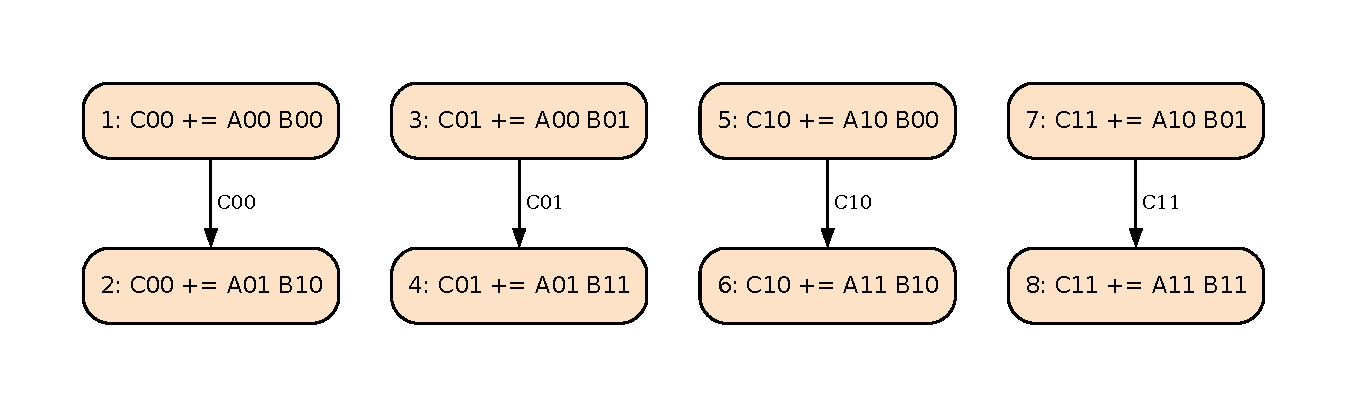
\includegraphics[width=0.95\linewidth]{./img/dag_gemm_2x2.pdf}
\end{center}

Four independent chains of two tasks: each \(C_{ij}\) is updated twice
(RAW), \(A\) and \(B\) are only read.
\end{frame}
\begin{frame}[label={sec:orga51e1ff}]{Work, critical path, granularity}
\begin{itemize}
\item \alert{Work} \(T_1\): \(NB^3\) block products.
\item \alert{Critical path} \(T_\infty\): \(NB\) block products (one per \(k\)).
\item \(T_1 / T_\infty = NB^2\) bounds the number of busy processors:
with \(NB = 2\), at most \alert{4} tasks at a time.
\end{itemize}

Granularity is a trade-off:
\begin{itemize}
\item larger \(NB\) \(\Rightarrow\) more parallelism, smaller tasks
(\(2\,BS^3\) flops each);
\item the cost per task is roughly constant, and GPUs need large blocks.
\end{itemize}

One of the few performance decisions left to the programmer.
\end{frame}
\begin{frame}[label={sec:org7f6138a},fragile]{Sequential Task Flow (STF)}
 \scriptsize
\begin{verbatim}
for (unsigned i = 0; i < NB; i++)            /* the loops do not change */
    for (unsigned j = 0; j < NB; j++)
        for (unsigned k = 0; k < NB; k++)
            starpu_task_insert(&gemm_cl,     /* was: gemm_block(...) */
                STARPU_R,  starpu_data_get_sub_data(A_h, 2, i, k),
                STARPU_R,  starpu_data_get_sub_data(B_h, 2, k, j),
                STARPU_RW, starpu_data_get_sub_data(C_h, 2, i, j), 0);
starpu_task_wait_for_all();
\end{verbatim}
\normalsize

\begin{itemize}
\item Submission is \alert{asynchronous}; the runtime builds the DAG on the fly.
\item Ready tasks run on any free unit while the main thread submits.
\item Sequential semantics, parallel execution.
\end{itemize}
\end{frame}
\begin{frame}[label={sec:orgbbcc472},fragile]{Hands-on 1 (15 min) --- first programs}
 Handout, section "Hands-on 1":
\begin{enumerate}
\item Build the examples with \texttt{make}.
\item Run \texttt{hello\_world} with 1, 2 and 4 workers.
\item Run \texttt{vector\_scal}: two tasks, one RW dependency.
\end{enumerate}
\end{frame}
\section{The StarPU runtime}
\label{sec:org66aeb27}

\begin{frame}[label={sec:orgdd92231}]{StarPU in the software stack}
\begin{center}
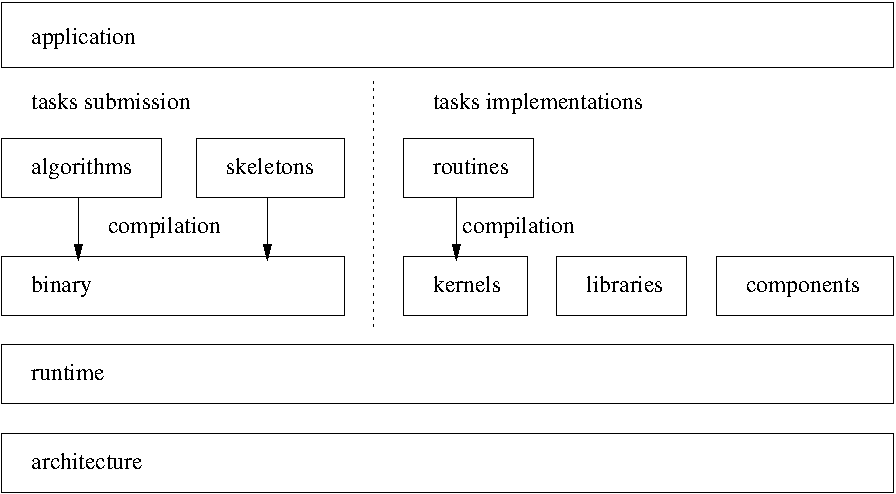
\includegraphics[height=0.6\textheight]{./img/stack-full.pdf}
\end{center}

C interface implementing STF; CPUs, CUDA, HIP, OpenCL, clusters with
StarPU-MPI. Developed at Inria Bordeaux (STORM team).
\end{frame}
\begin{frame}[label={sec:orgc81c9d1}]{Three components, three problems solved}
\begin{itemize}
\item \alert{Scheduler} (balancing): each ready task goes to a worker, chosen by
a scheduling policy --- from greedy to model-based.
\item \alert{Memory nodes} (transfers): main memory and each GPU memory; StarPU
tracks valid copies and moves blocks before a task needs them.
\item \alert{Workers} (pinning): one thread per CPU core, one per GPU (on a
dedicated core); one task at a time, no preemption.
\end{itemize}

Programmer-side abstractions: \alert{codelet} (a kind of task), \alert{data handle}
(a registered block), \alert{task} (a codelet applied to handles).
\end{frame}
\begin{frame}[label={sec:org25b8101},fragile]{Codelets and tasks}
 \scriptsize
\begin{verbatim}
void hello_cpu(void *buffers[], void *cl_arg)
{
    printf("Hello world from worker %d\n", starpu_worker_get_id());
    sleep(1);
}
struct starpu_codelet hello_cl = {
    .cpu_funcs = { hello_cpu }, .nbuffers = 0, .name = "hello",
};
int main(void)
{
    starpu_init(NULL);
    for (int i = 0; i < 4; i++)
        starpu_task_insert(&hello_cl, 0);
    starpu_task_wait_for_all();
    starpu_shutdown();
}
\end{verbatim}
\end{frame}
\begin{frame}[label={sec:org607fe8d},fragile]{Data handles and access modes}
 \scriptsize
\begin{verbatim}
struct starpu_codelet scal_cl = {
    .cpu_funcs = { scal_cpu }, .nbuffers = 1, .modes = { STARPU_RW },
};
starpu_data_handle_t vector_h;
starpu_vector_data_register(&vector_h, STARPU_MAIN_RAM,
                            (uintptr_t)vector, NX, sizeof(vector[0]));
starpu_task_insert(&scal_cl, STARPU_RW, vector_h,
                   STARPU_VALUE, &two, sizeof(two), 0);
starpu_task_insert(&scal_cl, STARPU_RW, vector_h,
                   STARPU_VALUE, &three, sizeof(three), 0);
starpu_data_unregister(vector_h);   /* data back in main memory */
\end{verbatim}
\normalsize

\begin{itemize}
\item StarPU infers RAW: the second task waits for the first.
\item Inside a task, \texttt{STARPU\_VECTOR\_GET\_PTR} gives the address \alert{in the
memory node where the task runs}.
\end{itemize}
\end{frame}
\begin{frame}[label={sec:orgf64b3cf},fragile]{Partitioning and coherence}
 \begin{itemize}
\item \alert{Filters} split a registered matrix into a grid of sub-handles:
\texttt{starpu\_matrix\_filter\_block} and \texttt{...\_vertical\_block}, applied with
\texttt{starpu\_data\_map\_filters()}.
\item Dependencies are computed \alert{per block}.
\item Coherence protocol, as in processor caches: several valid replicas
(one per memory node), invalidated on write, copied back lazily.
\item \texttt{starpu\_malloc()} gives pinned memory: asynchronous CPU--GPU
transfers overlapped with computation.
\item Implementations must read the layout (\texttt{STARPU\_MATRIX\_GET\_LD}) from
StarPU: a filtered block is not contiguous.
\end{itemize}
\end{frame}
\begin{frame}[label={sec:org9deff9d},fragile]{One codelet, several implementations}
 \scriptsize
\begin{verbatim}
static struct starpu_perfmodel gemm_model = {
    .type = STARPU_HISTORY_BASED, .symbol = "gemm",
};
static struct starpu_codelet gemm_cl = {
    .cpu_funcs = { gemm_cpu },
#ifdef STARPU_USE_CUDA
    .cuda_funcs = { gemm_cuda },        /* calls cublasSgemm */
    .cuda_flags = { STARPU_CUDA_ASYNC },
#endif
    .nbuffers = 3,
    .modes = { STARPU_R, STARPU_R, STARPU_RW },
    .model = &gemm_model,
};
\end{verbatim}
\normalsize

The scheduler picks the worker, hence the implementation, task by task.
\end{frame}
\begin{frame}[label={sec:orgb9538d2},fragile]{Schedulers and performance models}
 \small
\texttt{STARPU\_SCHED} selects the policy at runtime:
\begin{itemize}
\item \alert{Greedy} (\texttt{eager}, \texttt{lws} by default): first idle worker takes the
task; may give a large task to a slow core while the GPU is idle.
\item \alert{Model-based} (\texttt{dm}, \texttt{dmda}, inspired by HEFT): estimate on which
worker each task finishes first, with transfer times for \texttt{dmda}.
\end{itemize}

\texttt{STARPU\_HISTORY\_BASED} models record the duration of each
implementation per data size in \texttt{\textasciitilde{}/.starpu/sampling/}:
\begin{itemize}
\item the first runs calibrate (\texttt{STARPU\_CALIBRATE=1} forces it);
\item \texttt{starpu\_perfmodel\_display -s gemm}, \texttt{starpu\_perfmodel\_plot -s gemm}.
\end{itemize}

The static 80\% split becomes a task-by-task decision.
\end{frame}
\begin{frame}[label={sec:orgb7fecf9},fragile]{Hands-on 2 (30 min) --- the tiled matrix multiplication}
 Handout, section "Hands-on 2":
\begin{enumerate}
\item Run \texttt{gemm\_seq}, then complete the TODO of \texttt{gemm\_starpu\_todo.c}.
\item Run \texttt{gemm\_starpu 2048 2} and \texttt{2048 8}; compare GFlop/s.
\item Try \texttt{eager} and \texttt{dmda}; look at the performance model.
\item Watch the GPU demo on the instructor's machine.
\end{enumerate}
\end{frame}
\section{Observing task-based executions}
\label{sec:org942ef1f}

\begin{frame}[label={sec:orgfa98266}]{Why traces?}
\begin{itemize}
\item Time, speedup and efficiency are single numbers.
\item They do not say \alert{why} an execution is slow:
\begin{itemize}
\item the DAG lacks parallelism?
\item workers wait for data transfers?
\item some tasks take longer than expected?
\item the runtime itself is a bottleneck?
\end{itemize}
\item Answering requires looking at what happened: \alert{execution traces}.
\end{itemize}
\end{frame}
\begin{frame}[label={sec:org566d1bf},fragile]{Recording a trace}
 \begin{itemize}
\item StarPU built with FxT (true in the tutorial image).
\item At runtime: \texttt{STARPU\_FXT\_TRACE=1}, files in \texttt{STARPU\_FXT\_PREFIX},
written at \texttt{starpu\_shutdown()}.
\item \texttt{STARPU\_GENERATE\_TRACE=1} also converts them (\texttt{paje.trace},
\texttt{tasks.rec}, \texttt{dag.dot}) in the current directory.
\end{itemize}

Two containers today: StarPU records and converts, StarVZ
(\texttt{docker.io/viniciusvgp/starvz}) analyzes.
\end{frame}
\begin{frame}[label={sec:org6b12252},fragile]{The StarVZ workflow}
 \begin{itemize}
\item \alert{Phase 1} (shell): Paje trace \(\rightarrow\) compact \texttt{.parquet}
files describing tasks, workers, handles and the DAG.
\item \alert{Phase 2} (R): read them and build a figure of synchronized panels,
selected by a YAML file.
\end{itemize}

\scriptsize
\begin{verbatim}
starvz --use-paje-trace --keep --phase1 trace_nb8/
Rscript starvz_compare.R starvz_compare.yaml trace_nb2 trace_nb8 out.png
\end{verbatim}
\end{frame}
\begin{frame}[label={sec:orga615554}]{Reading a space-time diagram}
\begin{center}
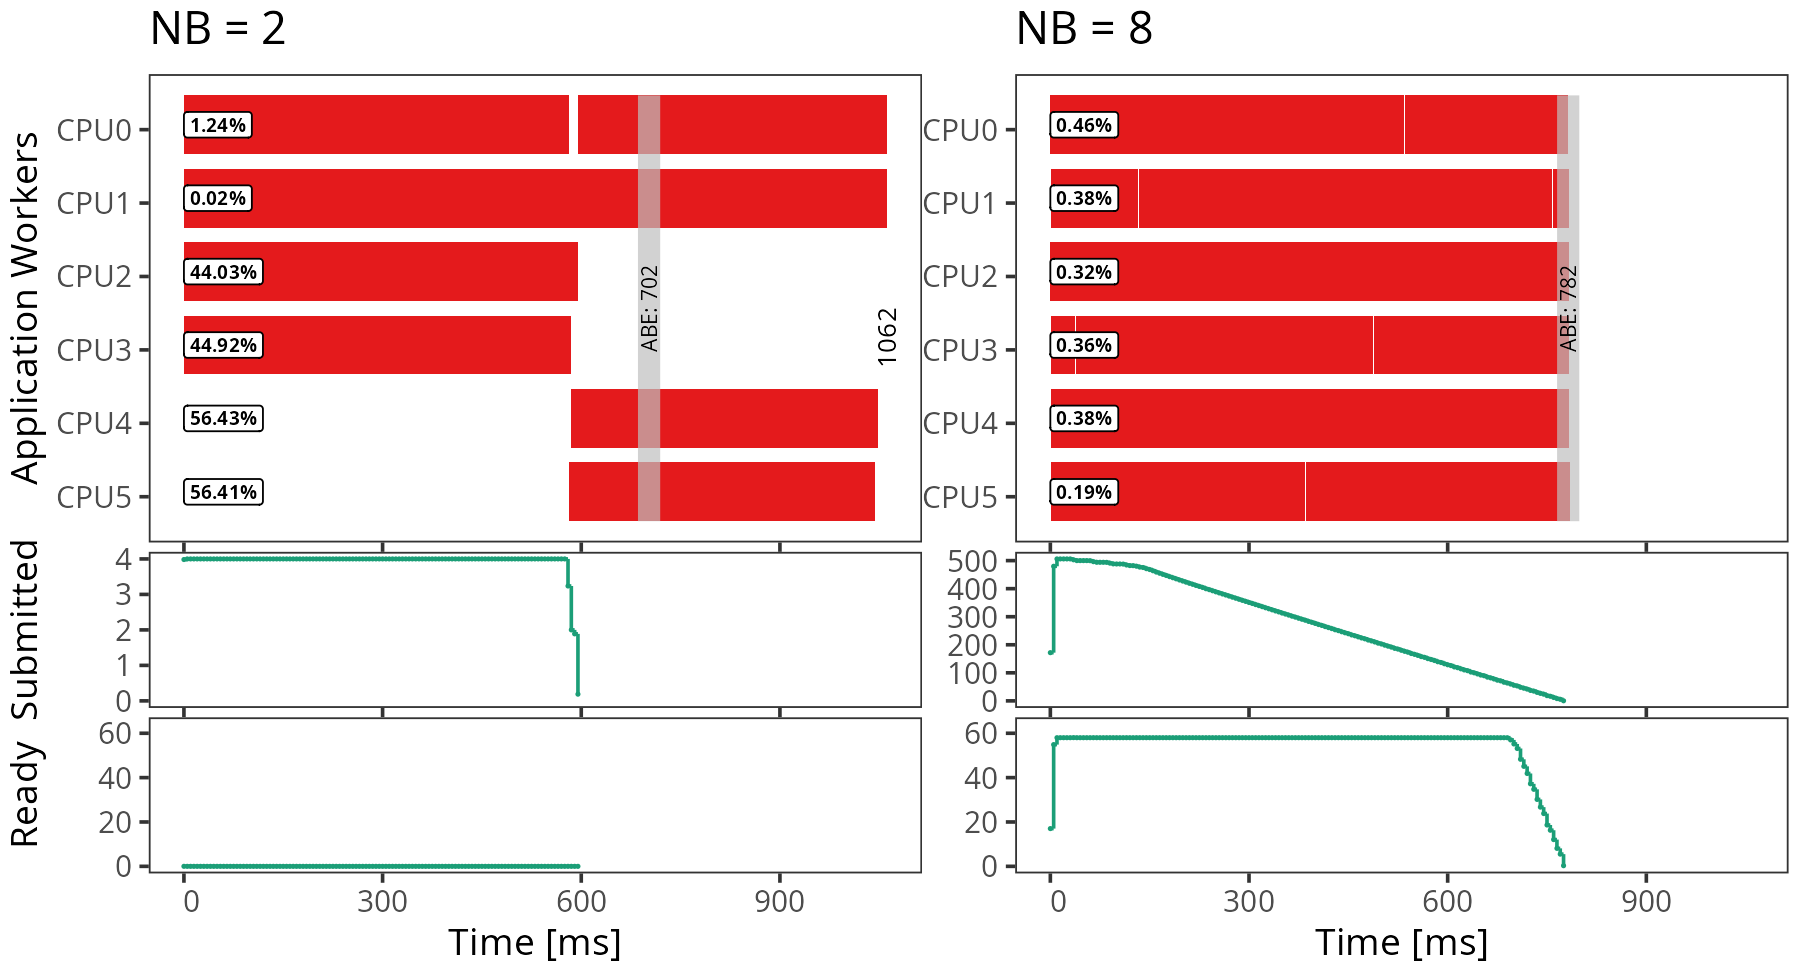
\includegraphics[height=0.62\textheight]{./img/starvz_gemm_nb2_nb8.png}
\end{center}

Rows: workers; rectangles: tasks; left: idleness; gray band: ABE lower
bound (ignores dependencies); bottom: submitted and ready tasks.
\end{frame}
\begin{frame}[label={sec:orgd68e70a}]{What to look for}
\begin{itemize}
\item Gaps \alert{and} few ready tasks: the DAG lacks parallelism (\(NB = 2\)).
\item Gaps \alert{while} many tasks are ready: runtime or data transfers (more
panels on memory nodes and transfers).
\item Tasks much longer than others of the same type: \alert{outliers}, often
interference.
\item On a heterogeneous node: did the scheduler keep CPUs \alert{and} GPUs
busy?
\end{itemize}
\end{frame}
\begin{frame}[label={sec:orgc97dbe2},fragile]{Hands-on 3 (25 min) --- traces and StarVZ}
 Handout, section "Hands-on 3":
\begin{enumerate}
\item Record traces of \texttt{gemm\_starpu 2048 2} and \texttt{2048 8}.
\item Phase 1 in the StarVZ container.
\item Plot both traces side by side; answer the questions.
\item Look at the instructor's CPU+GPU traces (\texttt{eager} vs. \texttt{dmda}).
\end{enumerate}
\end{frame}
\section{Closing}
\label{sec:org9555f80}

\begin{frame}[label={sec:org5acdfcd},fragile]{CPU+GPU: \texttt{eager} vs. \texttt{dmda} (instructor's machine)}
 \begin{center}
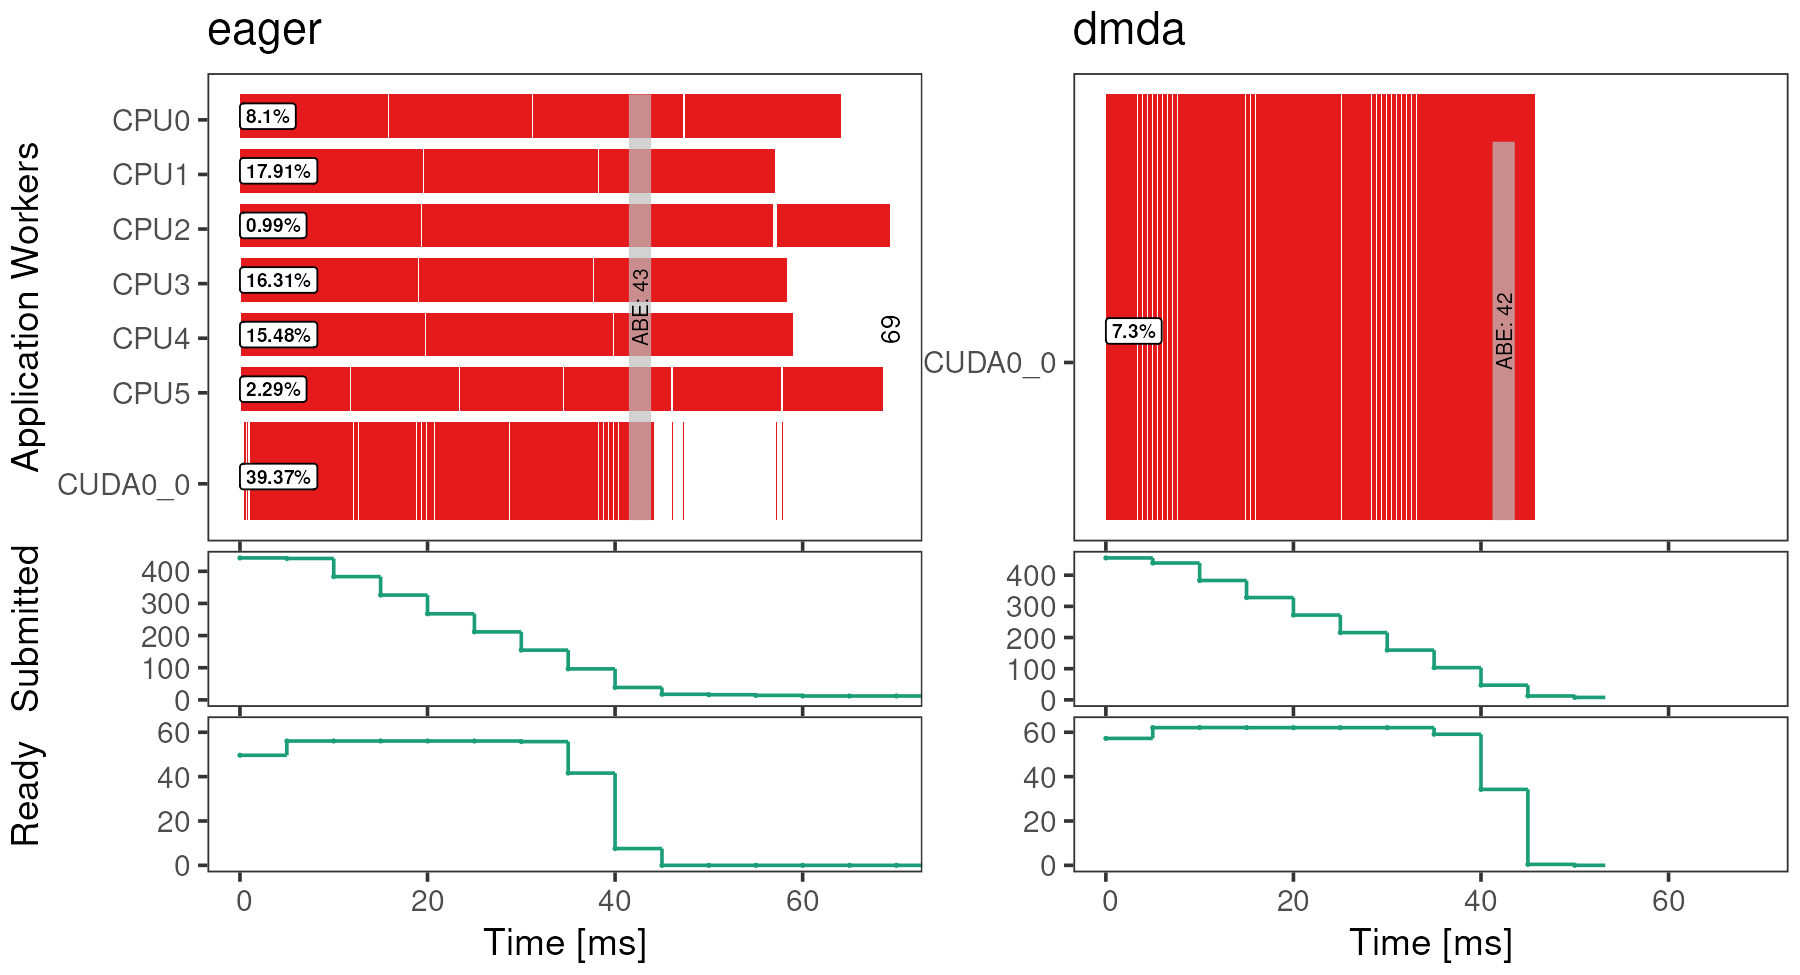
\includegraphics[height=0.68\textheight]{./img/starvz_gpu_eager_dmda.png}
\end{center}

Same binary, 6 CPU workers + 1 GPU, \(N = 2048\), \(NB = 8\).
\end{frame}
\begin{frame}[label={sec:orga238979},fragile]{What we left out}
 \begin{itemize}
\item Distributed execution with StarPU-MPI (same STF model, across nodes).
\item Reductions and commutative accesses (relaxing RW dependencies).
\item Advanced schedulers (\texttt{dmdas}, \texttt{heteroprio}, \ldots{}), HIP and OpenCL.
\end{itemize}

Material:
\begin{itemize}
\item Book chapter and this repository: \url{https://github.com/schnorr/starpu-tutorial}
\item StarPU documentation and tutorials: \url{https://starpu.gitlabpages.inria.fr/}
\item StarVZ: \url{https://github.com/schnorr/starvz}
\end{itemize}

Questions?
\end{frame}
\end{document}
